\documentclass[12pt]{article}
\usepackage[a4paper]{geometry}
%\userpackage[top=1 in, bottom=1.25 in, left=1.1 in, rigth=1.1 in] {geometry}
%\usepackage[paperwidth=17cm, paperheight=22.5cm, bottom=2.5cm, right=2.5cm]{geometry}
\usepackage[utf8]{inputenc}
%\usepackage[a4paper, top=2.5cm, bottom=2.5cm, left=2.2cm, right=2.2cm]
%{geometry}
%\usepackage[myheadings]{fullpage}
\usepackage{fancyhdr}
\usepackage{lastpage}
%\usepackage{float}
\usepackage{graphicx, wrapfig, subcaption, setspace, booktabs}
\usepackage{graphicx}
\usepackage[T1]{fontenc}
\usepackage[font=small, labelfont=bf]{caption}
%\usepackage{fourier}
\usepackage[protrusion=true, expansion=true]{microtype}
\usepackage[english]{babel}
\usepackage{sectsty}
\usepackage{url, lipsum}
\usepackage[T1]{fontenc}
\usepackage{icomma}
\usepackage{siunitx}
\usepackage{ragged2e}
\usepackage{amsmath}
\usepackage{comment}
\usepackage{enumerate}
%\usepackage{changepage}
\usepackage{anysize}




\newcommand{\HRule}[1]{\rule{\linewidth}{#1}}
\onehalfspacing
\setcounter{tocdepth}{5}
\setcounter{secnumdepth}{5}

%-------------------------------------------------------------------------------
% HEADER & FOOTER
%-------------------------------------------------------------------------------


\begin{comment}
-Udledninger
$$
\begin{aligned}
\end{aligned}
$$

-Opgavetekst
\begin{figure}[H]
\includegraphics[width=0.5\textwidth]{"path"}
\end{figure} 


-Opgave billede med tekst
\begin{figure}[H]
\caption{"Billedtekst"}
\includegraphics[width=0.5\textwidth]{"path"}
\end{figure} 

-Værdier
$\\
$


\end{comment}
\begin{document}

\begin{titlepage}

\title{ \normalsize 
		%\begin{figure}
        \begin{center}
        
\includegraphics[height=6cm]{Logo.jpg}
        \end{center}
       % \end{figure}
        \LARGE \textsc{\textbf{Universidad De Sonora}} \\ \bigskip
		\Large División de Ciencias Exactas y Naturales \\
        Licenciatura en Física \\ \bigskip
        \bigskip
        Física Computacional I
		\\ [0.1cm]  
		\HRule{2pt} \\
		\Large \textbf{{Actividad 8}} \\
        \textit{\textbf{"Solución de Ecuaciones Diferenciales Ordinarias con Python"}}
		\HRule{2pt} \\
		\normalsize \vspace*{0.001\baselineskip}}
        
\date{\bigskip \Large  \hspace*{\fill} Hermosillo, Sonora a marzo 14 de 2021}

        
\author{
		\Large\textbf{ Ismael Espinoza Arias} \\ \bigskip
        \\ \bigskip
       \Large Profesor Carlos Lizárraga Celaya}
       \end{titlepage}
       \maketitle
       
       
%-----------------------------------------------------------


\section*{Introducción y Antecedentes}
En esta actividad, trata de la octava práctica de la materia de Física Computacional I, en esta ocasión realizamos un análisis del Oscilador de Van der Pol, que es como un caso ams especial del oscilador armónico, que es parte de las actividades anteriores, es un oscilador con amortiguamiento no lineal.\\

Balthasar Van der Pol (27 de enero de 1889 - 6 de octubre de 1959) fue un físico holandés. Estudió física en Utrecht , y en 1920 obtuvo su doctorado (PhD).Se unió a Philips Research Labs en 1921, donde trabajó hasta su retiro en 1949. Sus intereses principales eran la propagación de ondas de radio , la teoría de los circuitos eléctricos y la física matemática . El oscilador de Van der Pol , uno de los modelos más utilizados de no lineal auto-oscilación , lleva su nombre. Fue galardonado con el Instituto de Ingenieros de Radio (ahora el IEEE ) Medalla de Honor en 1935. \\

La ecuación de Van der Pol tiene una larga historia de uso en las ciencias físicas y biológicas. Más adelante se presentará la síntesis correspondiente al temas, además de las gráficas de los ejemplos del oscilador y un análisis de los resultados obtenidos. 


%-----------------------------------------------------------


\section*{Modelo de Van der Pol}
En dinámica , el oscilador der Pol Van es un oscilador con amortiguamiento no lineal. Se desarrolla en el tiempo de acuerdo con la ecuación diferencial de segundo orden :\\

\centerline{$\displaystyle \frac{d^2x}{dt^2} - \mu (1-x^2) \frac{dx}{dt} +x = 0$}
$ $\\
donde $x$ es la coordenada de posición, que es una función del tiempo $t$ , y $\mu$ es un parámetro escalar que indica la no linealidad y la fuerza de la amortiguamiento.


%-----------------------------------------------------------


\subsection*{Historia}
El oscilador Van der Pol fue propuesto originalmente por el ingeniero eléctrico y físico holandés Balthasar van der Pol mientras trabajaba en Philips. Van der Pol encontró oscilaciones estables, que luego denominó relajaciones - oscilaciones y ahora se conocen como un tipo de ciclo límite en circuitos eléctricos que emplean tubos de vacío. Cuando se hacían funcionar a estos circuitos cerca de su ciclo límite, la señal entra en fase con la corriente, y con ayuda de uno de los colegas de Van der Pol, Van de Mark, encontraron que para ciertas frecuencias aparecía un ruido irregular siempre cerca de las frecuencias de acoplamiento, que más tarde se descubrió que era el resultado de un caos determinista. \\

La ecuación de Van der Pol tiene una larga historia de uso en las ciencias físicas y biológicas. Por ejemplo, en biología, Fitzhugh y Nagumo extendieron la ecuación en un campo plano como un modelo para los potenciales de acción de las neuronas. La ecuación también se ha utilizado en sismología para modelar las dos placas en una falla geológica, y en estudios de la fonación para modelar los osciladores de las cuerdas vocales derecho e izquierdo.


%-----------------------------------------------------------


\subsection*{Forma Bidimensional}
El teorema de Liénard se puede usar para demostrar que el sistema tiene un ciclo límite. Aplicando la transformación Liénard $\displaystyle y = x - \frac{x^3}{3}- \frac{\dot x}{\mu}$, donde el punto indica la derivada del tiempo, el oscilador de Van der Pol se puede escribir en su forma bidimensional: \\

\centerline{$\displaystyle \dot x = \mu (x- \frac{1}{3}x^3 - y) $}
$ $\\
\centerline{$\displaystyle \dot y= \frac{1}{\mu}x$}\\

Otra forma comúnmente utilizada basada en la transformación $y = \dot x$ lleva a:\\
\centerline{$\dot x = y$}\\
\centerline{$\dot y = \mu (1-x^2)y-x$}


%-----------------------------------------------------------


\subsection*{Oscilador Sin Forzamiento}
Existen varias características interesantes de este oscilador para ciertas circunstancias:\\

$\to$ Cuando $\mu=0$, es decir, no hay amortiguamiento, la ecuación se convierte en $\displaystyle \frac{d^2x}{dt^2}+x = 0$ que es una forma de un oscilador armónico simple y siempre hay conservación de energía.\\

$\to$ Cuando $\mu>0$, el sistema entrará en un ciclo límite. Cerca del origen el sistema es inestable y, lejos del origen, el sistema está amortiguado.\\

$\to$ El oscilador Van der Pol no tiene una solución analítica exacta. Dicha solución para el ciclo límite existe si $f(x)$ en la ecuación de Lienard es una función constante por partes.


%-----------------------------------------------------------


\subsection*{Hamiltoniano para el Oscilador Van der Pol}
se puede escribir un formalismo hamiltoniano independiente del tiempo para el oscilador Van der Pol aumentándolo a un sistema dinámico autónomo tetradimensional usando una ecuación diferencial no lineal de segundo orden auxiliar de la siguiente manera:\\
\centerline{$\displaystyle \ddot x - \mu (1-x^2)\dot x+x=0 $}
\centerline{$\displaystyle \ddot y + \mu (1-x^2)\dot y+y=0 $}
Se puede demostrar que el Hamiltoniano $H$ para este sistema de ecuaciones es:\\
\centerline{$ H(x,y,p_x,p_y) = p_x p_y +xy -\mu (1-x^2)yp_y$}
donde $p_x$ y $p_y$ son los momentos conjugados correspondientes a $x$ y $y$ , respectivamente. Esto puede, en principio, conducir a la cuantificación del oscilador Van der Pol.


%-----------------------------------------------------------


\subsection*{Oscilador con Forzamiento}
El oscilador forzado o impulsado de Van der Pol toma la función "original" y agrega una función de conducción $A \sin ( \omega t )$ para dar una ecuación diferencial de la forma:\\

\centerline{$\displaystyle \frac{d^2x}{dt^2} - \mu (1-x^2) \frac{dx}{dt} +x-A \sin ( \omega t )  = 0$}
$ $\\
donde $A$ es la amplitud  o desplazamiento, de la función de onda y $\omega$ es su velocidad angular.


%-----------------------------------------------------------


\subsection*{Circuito Eléctrico - Caos Determinista}
Para hacer los circuitos eléctricos descritos por la ecuación de Van der Pol, los elementos del circuito activo con la propiedad cúbica no lineal, $i = \phi(v)=\gamma v^3-\alpha v$, se requieren, donde $i$ y $v$ son corriente y voltaje, respectivamente. En la década de 1920, Van der Pol construyó el oscilador utilizando el triodo o el tetrodo. Después de que Reona Esaki inventó el diodo túnel en 1957, hacer el oscilador de Van der Pol con circuitos eléctricos se hizo mucho más simple.
Usando el diodo del túnel con relación entrada-salida, la ecuación se puede reescribir como:\\

\centerline{$\displaystyle \ddot V - \frac{1}{C}(\alpha-3\gamma V^2)\dot V+\frac{1}{LC}V=0$}
$ $\\
Se sabe que el caos se puede encontrar en el sistema cuando la no linealidad del sistema es suficientemente fuerte. Van der Pol y Van der Markconsideraron un circuito eléctrico compuesto por una resistencia, una capacitancia y una lámpara Ne, y escucharon la respuesta del sistema al insertar los receptores telefónicos en su circuito. Además de los comportamientos de bloqueo, escucharon ruidos irregulares antes de que el período del sistema salte al siguiente valor. Afirmaron que este ruido es un fenómeno subsidiario, pero hoy se cree que escucharon el caos determinista en 1927 antes que Yoshisuke Ueda y Edward Lorenz.


%-----------------------------------------------------------


\section*{Exploración - Soluciones del Modelo en el Espacio Fase}
Para reproducir las gráficas del artículo de Wikipedia, fue necesario (como en las actividades pasadas) definir un vector que almacene el sistema de ecuaciones diferenciales, asi como crear valores del tiempo, agregar condiciones iniciales, resolver el sistema de ecuaciones diefrenciales con la función odeint y que todo esto se guarde en un archivo para que pueda leerse. A continuación la sección de código utilizada y las gráficas generadas.
\begin{center}
    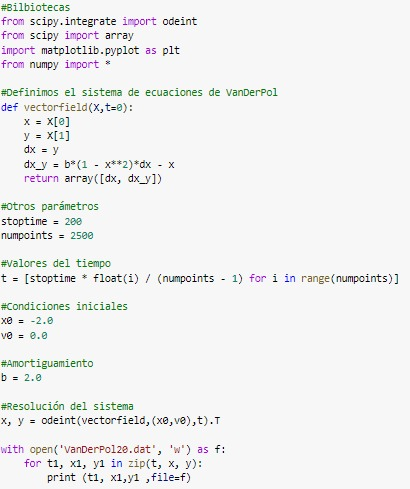
\includegraphics[height=15cm]{O1.jpeg}\\
\end{center}
\begin{center}
    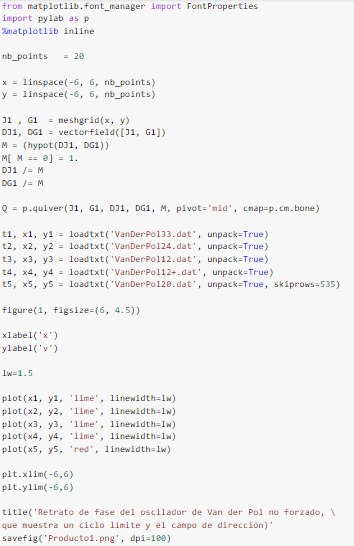
\includegraphics[height=18cm]{O2.jpeg}\\
\end{center}
Para generar la gráfica fue necesario crear 4 archivos, ya que son 4 osciladores con distintas condiciones iniciales. Ahora se introdujo tambien lo que es el campo vectorial, que son las flechas que apuntan en dirección de la derivada. Fue con la ayuda de una función "quiver" de matplot que se utiliza para graficar vectoreres, pero para ello, se genera una cuadricula donde se almacenan los valores necesarios para la graficación del campo.\\

La gráfica obtenida es la siguiente:
\begin{center}
    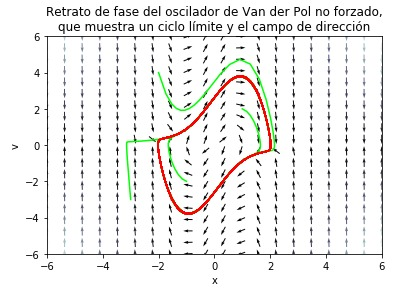
\includegraphics[height=7.5cm]{2.jpeg}\\
\end{center}

Para la segunda gráfica solo se crearon archivos con diferente coeficiente de amortiguamiento, el código es el siguiente:
\begin{center}
    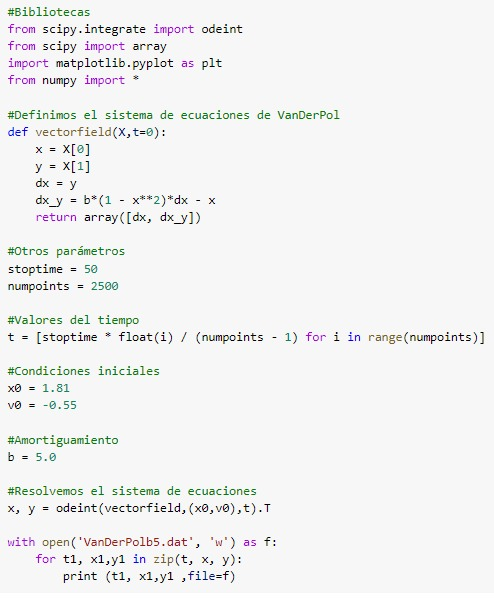
\includegraphics[height=14cm]{O3.jpeg}\\
\end{center}
\begin{center}
    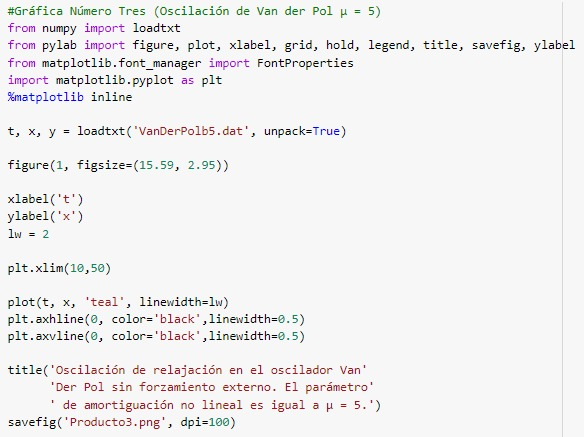
\includegraphics[height=13cm]{O4.jpeg}\\
\end{center}

A continuación se presenta la gráfica y en su parte derecha los valores de amortiguamiento correspondientes. (Fácil de visualizar por los colores)
\begin{center}
    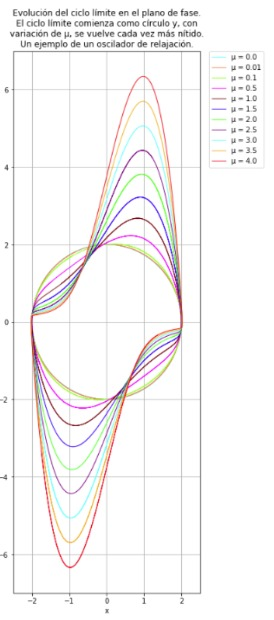
\includegraphics[height=20cm]{3.jpeg}\\
\end{center}
Para la tercera gráfica solo fue necesario un archivo, ya que solo es un oscilador con coeficiente de amortiguamiento igual a 5.
\begin{center}
    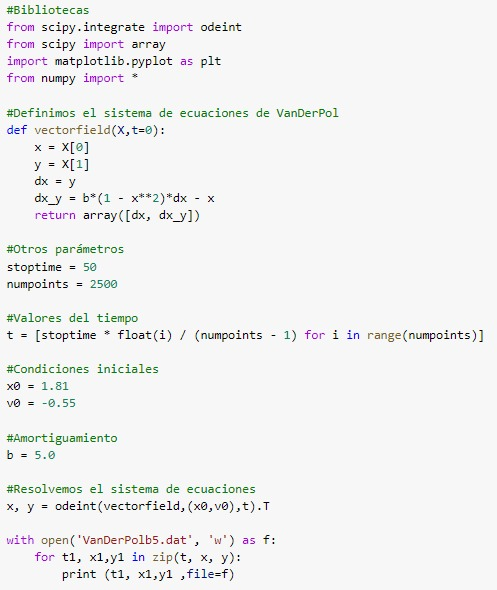
\includegraphics[height=12cm]{O5.jpeg}\\
\end{center}
\begin{center}
    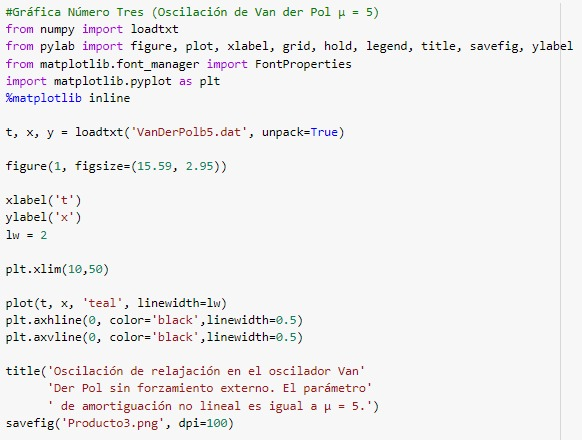
\includegraphics[height=10cm]{O6.jpeg}\\
\end{center}
La gráfica obtenida es:
\begin{center}
    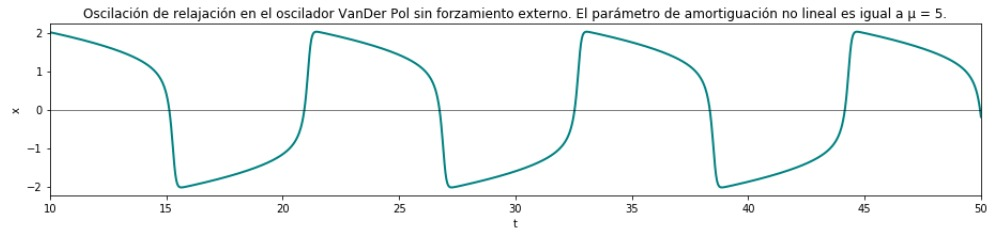
\includegraphics[height=3.15cm]{4.jpeg}\\
\end{center}

Por último, la ultima gráfica que se presenta en al articulo es la de un oscilador forzado con valores de $\mu$ = 8.53, $A$ = 1.2 y $\omega = 2\pi/ 10$. \\

Al vector que almacena la ecuación solamente se le agregó el valor de forzamiento anteriormente indicado, y se grafico la posición contra el tiempo.\\

Primaramente vamos a presentar la sección de código utilizada.
\begin{center}
    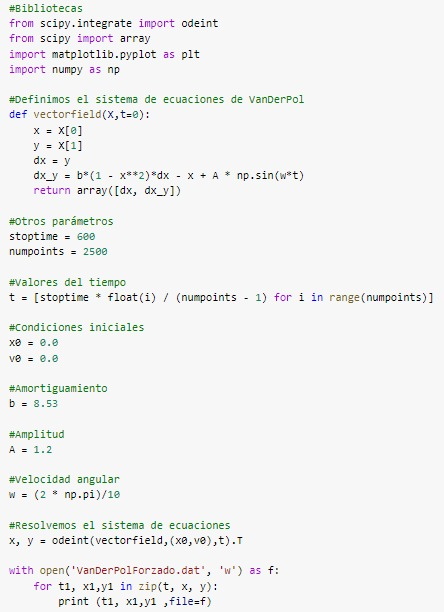
\includegraphics[height=16cm]{O7.jpeg}\\
\end{center}
\begin{center}
    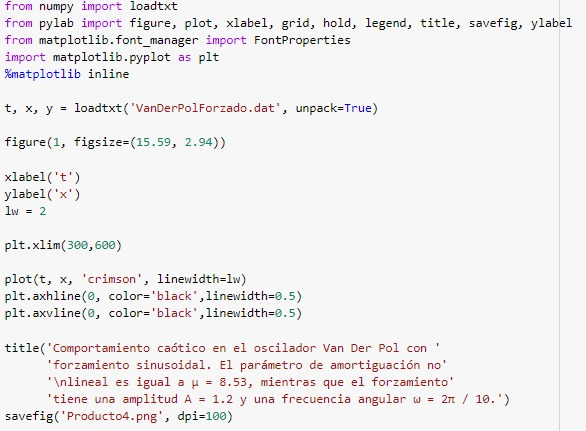
\includegraphics[height=12cm]{O8.jpeg}\\
\end{center}
\newpage
La gráfica obtenida es:
\begin{center}
    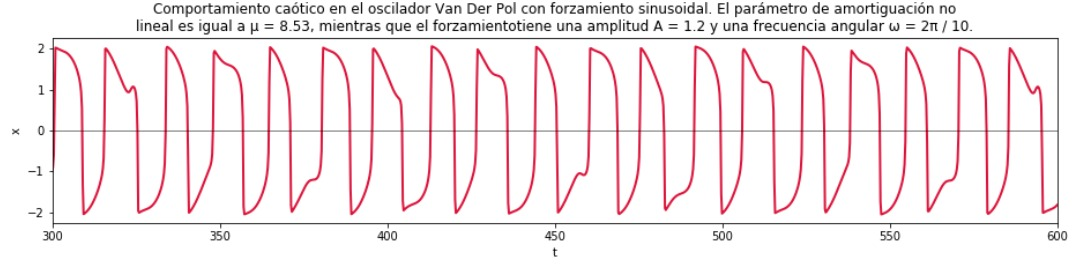
\includegraphics[height=3.15cm]{1.jpeg}\\
\end{center}


%-----------------------------------------------------------


\section*{Resultados y Discusión}
Como nos pudimos dar cuenta las gráficas se hacen de una distinta, es decir, dependen de ciertas cosas para realizarlas.
El primer ejercicio, donde como producto se genera un gráfica de campo vectorial, no indica que a pesar de las condiciones iniciales, teniendo el mismo factor de amortiguamiento, podrán tener un mismo ciclo límite. Es notorio también que las flechas del campo que estan alejadas solo se dirigen hacia valores positivos y negativos de $y$ y las flechas cercanas al ciclo límite siguen una curva.

La tercera y cuarta gráfica nos muestran la posición contra el tiempo del oscilador, uno que presenta forzamiento y otro que no presenta forzamiento. Al hacer una comparación con existir forzamiento se crean cambios bruscos y cunado no existe tal forzamiento se comportan de una forma casi periódica.


%-----------------------------------------------------------


\section*{Conclusiones del Estudio}
Se desprende que el oscilador de Van der Pol tiene como punto de equilibrio siempre el origen, el cual es un nodo o espiral,
inestables en todos los casos; favorece las oscilaciones
pequeñas y amortigua las grandes; se comporta como un sistema de Liénard, ya que tiene una única trayectoria cerrada que rodea al origen y hacia ella tienden en espiral todas las demás
trayectorias, asegurándose con esto que hay un ciclo límite estable en el espacio fase.Como se menciono anteriormente en el reporte, Van der Pol, al estudiar el oscilador forzado que lleva su nombre, descubrió lo que viene siendo un resultado del caos determinista. \\

Usar Python por medio de Jupyter Lab son herramientas de uso fácil para examinar información y a través de sus productos como los archivos y las gráficas encontrar nueva información para solucionar problemas de manera númerica, que sin este tipo de herramientas seria una tarea bastante larga y complicada.


%-----------------------------------------------------------


\section*{Bibliografía}
\begin{itemize}
\item Matplotlib: lotka volterra tutorial — SciPy Cookbook documentation. (2018). Scipy-cookbook.readthedocs.io. 
Recuperado el 13 de Abril de 2018 desde:\\
http://scipy-cookbook.readthedocs.io/items/LoktaVolterraTutorial.html

\item Van der Pol oscillator. (2018). Recuperado el 13 de Abril de 2018 desde:\\ https://en.wikipedia.org/wiki/Van\_der\_Pol\_oscillator

\item Van der poll oscillator. (2018). Recuperado el 13 de Abril desde: \\
http://www.scholarpedia.org/article/Van\_der\_Pol\_oscillator
\end{itemize}


%-----------------------------------------------------------


\section*{Apéndice}
\begin{enumerate}
\item Este ejercicio pareciera similar al desarrollado en las actividades 6 y 7. ¿Qué aprendiste nuevo?\\
\textit{Aprendí como generar un campo vectorial para la solucín del sistema de ecuaciones diferenciales y como cambiar las dimensiones en las imágenes para que sean reproducciones tal cual de los artículos.}
\item ¿Qué fue lo que más te llamó la atención del oscilador de Van der Pol?\\
\textit{Los ciclos límite y el cambio repentino y brusco en el comportamiento cuando existe o no el forzamiento.}
\item Has escuchado ya hablar de caos. ¿Por qué sería importante estudiar este oscilador?\\
\textit{No habia escuchado pero por lo que leí, este oscilador podría ser una base para el estudio del mismo.}
\item ¿Qué mejorarías en esta actividad?\\
\textit{Tratar de referenciar con información mas digerible rapidamente, podria decir.}
\item ¿Algún comentario adicional antes de dejar de trabajar en Jupyter con Python?\\
\textit{Es un lenguaje de los más usados y muy extenso, pero presiento que conocí una parte valiosa de él.}
\item Cerramos la parte de trabajo con Python ¿Que te ha parecido?\\
\textit{Fue una buena experiencia trabajar con este lenguaje, pues, es muy fácil de manejar a diferencia de otros, y logra cosas que otros no pueden o bien sea una tarea dificil, tal es el caso de métodos numéricos, graficación, solución de sistemas de ecuaciones diferenciales, etc. Todo con la ayuda de sus bibliotecas.}
\end{enumerate}

\end{document}